%Adapted by Evan Lim. Many thanks to Ivan Griffin for the original work, and to Janosh Riebessel, whose remix I have modified. Also, credits to David Carlisle for the \specialcell command.
\documentclass[tikz,border=10mm]{standalone}
\usetikzlibrary{shapes,calc}
\usepackage{amsmath}
\usepackage{amssymb}
\usepackage{amsfonts}
\newcommand{\specialcell}[2][c]{
	\begin{tabular}[#1]{@{}c@{}}#2\end{tabular}}
\newcommand{\ElemLabels}[5]{
	\begin{minipage}{1.8cm}
	\centering
		{\textbf{#1}\hfill #4}%
		\vspace{2mm}
		\linebreak
		{\textbf{#3}}%
		\linebreak {{#5}} \linebreak
		{{#2}}
  \end{minipage}
}
\newcommand{\ElemLabelNEN}[4]{
  \begin{minipage}{1.8cm}
	\centering
		{\textbf{#1}}%
		\vspace{2mm}
		\linebreak
		\textbf{#3}%
		\linebreak
		{#4}
		\linebreak {#2}
  \end{minipage}
}
\newcommand{\NaturalElem}[5]{\ElemLabels{#1}{#2}{\LARGE {#3}}{#4}{#5}}
\newcommand{\SyntheticElem}[4]{\ElemLabelNEN{#1}{#2}{\color{white}{\LARGE {#3}}}{#4}}
\newcommand{\SyntheticElemToo}[4]{\ElemLabelNEN{#1}{#2}{\color{gray}{\LARGE {#3}}}{#4}}
\newcommand{\SyntheticElemEN}[5]{\ElemLabels{#1}{#2}{\color{white}{\LARGE {#3}}}{#4}{#5}}
\newcommand{\up}[1]{\textsuperscript{#1}}
\begin{document}
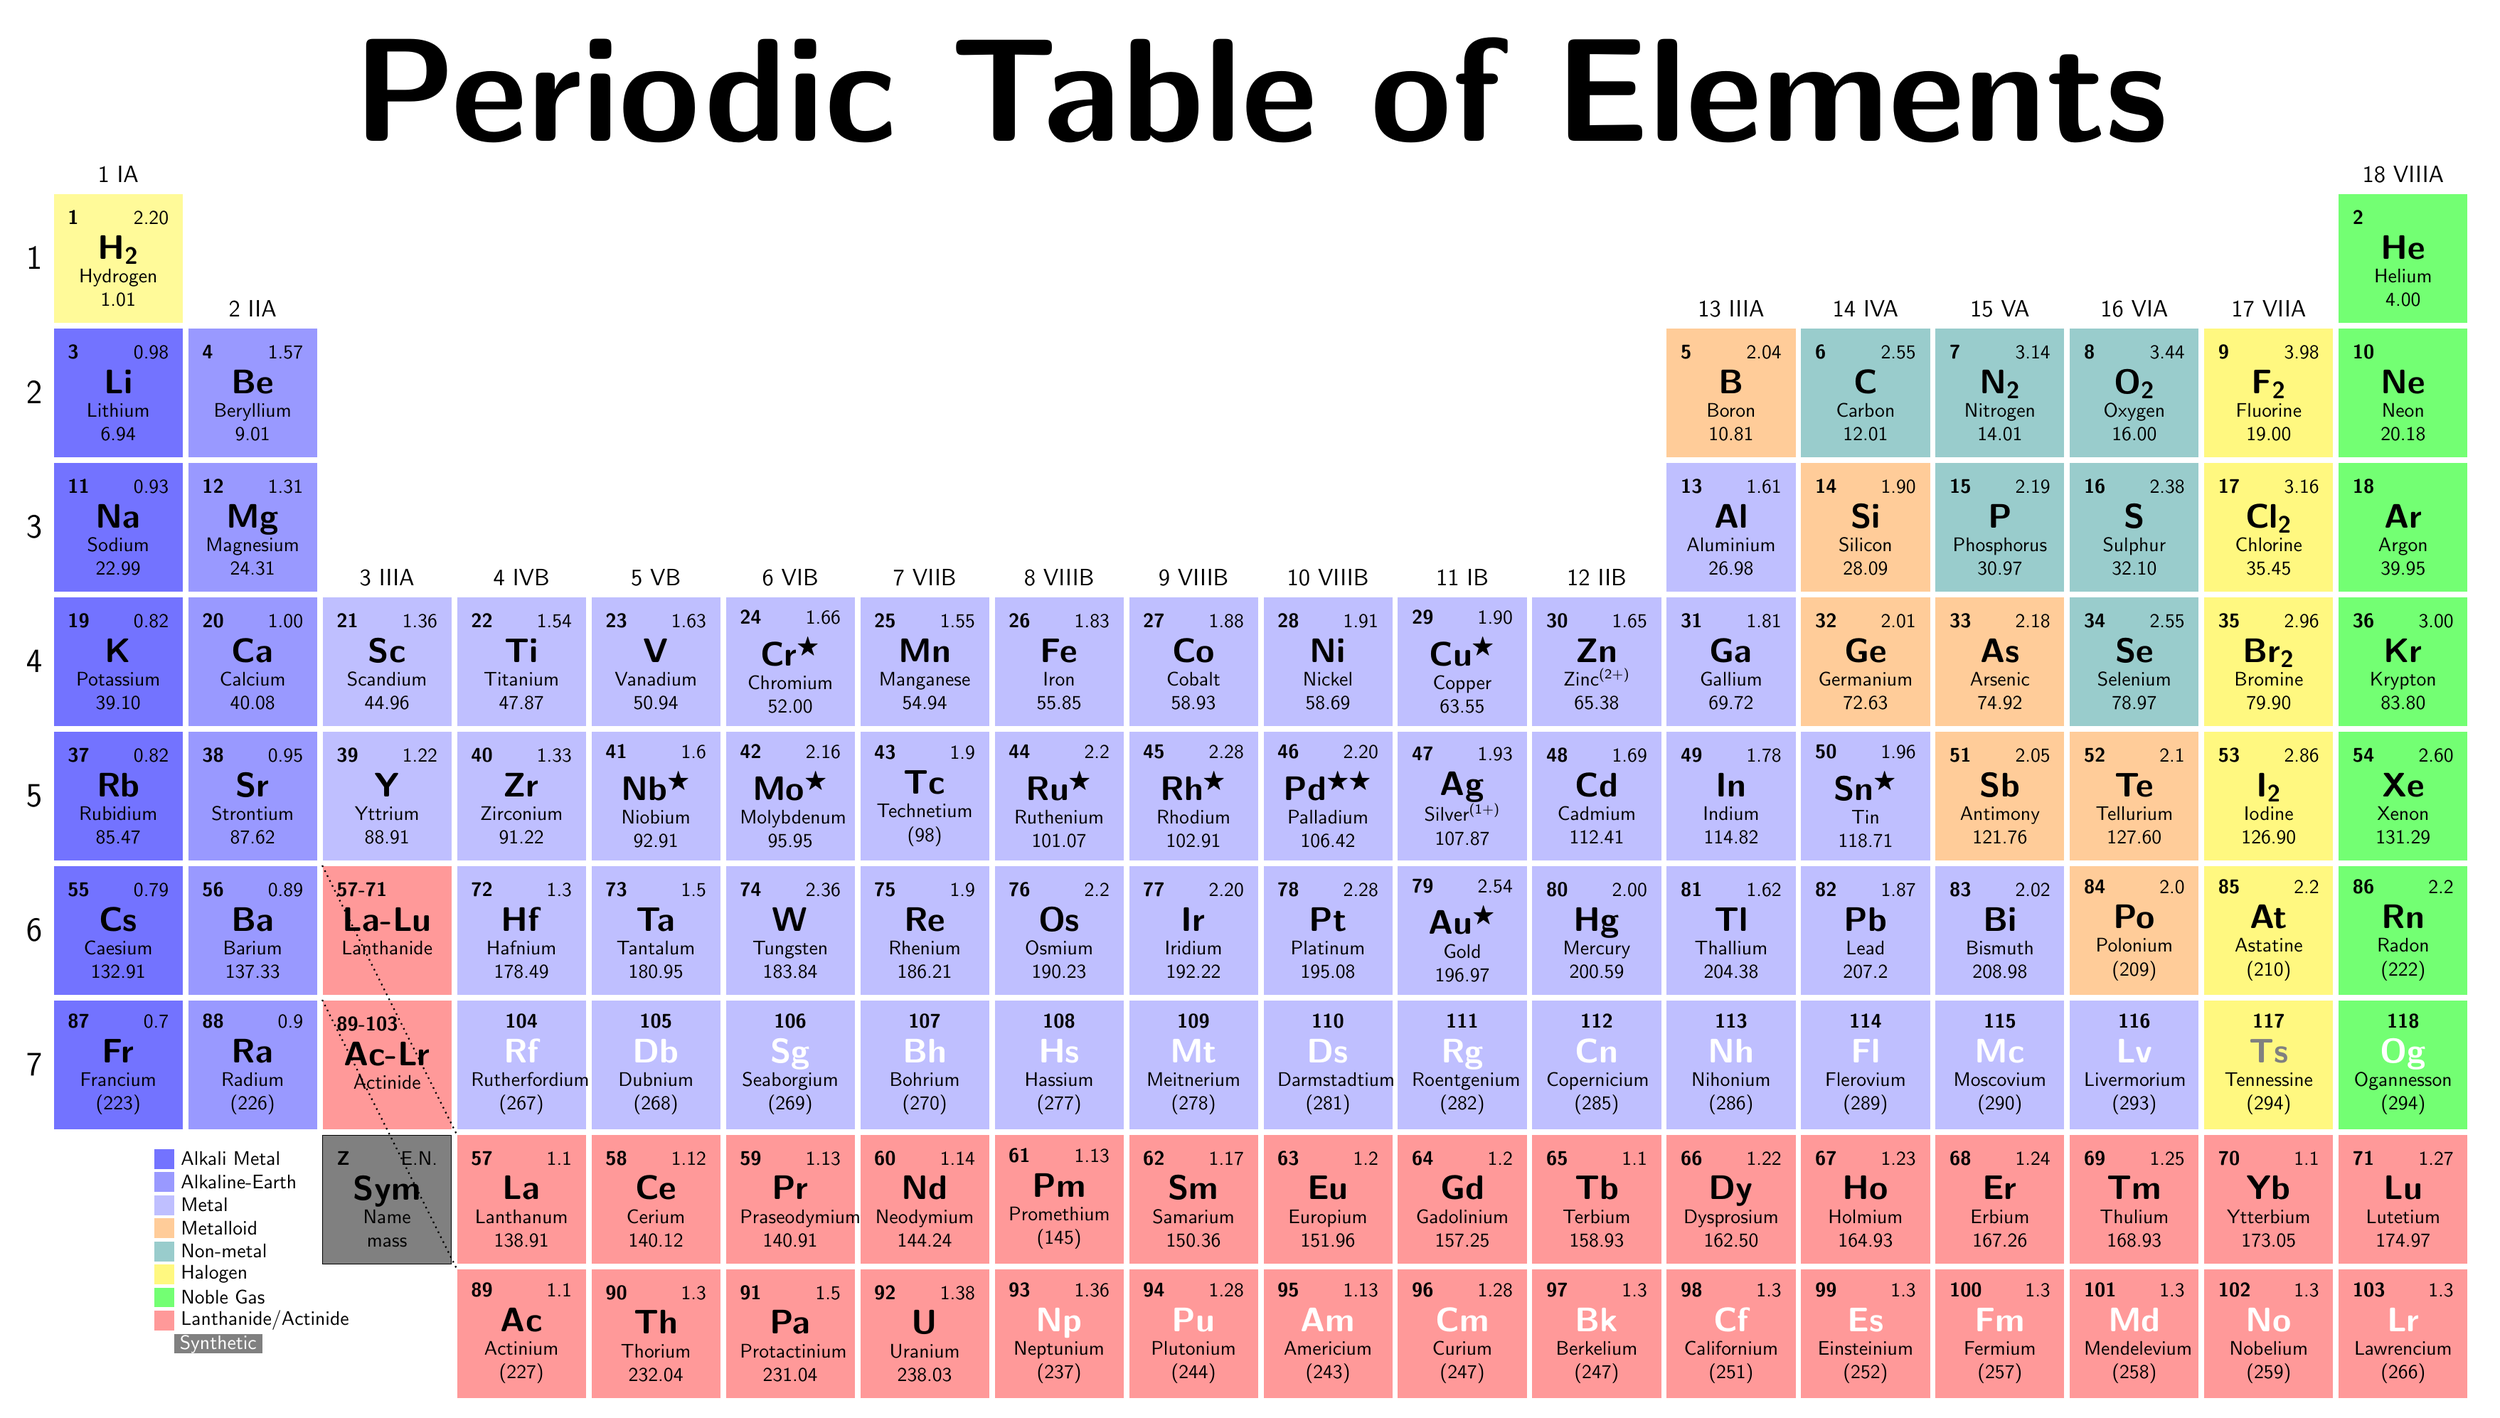
\begin{tikzpicture}[font=\sffamily]

  % Fill Color Styles
	\tikzstyle{ElementFill} = [fill=yellow!40]
	\tikzstyle{AlkaliMetalFill} = [fill=blue!55]
	\tikzstyle{AlkalineEarthMetalFill} = [fill=blue!40]
	\tikzstyle{MetalFill} = [fill=blue!25]
	\tikzstyle{MetalloidFill} = [fill=orange!40]
	\tikzstyle{NonmetalFill} = [fill=teal!40]
	\tikzstyle{HalogenFill} = [fill=yellow!50]
	\tikzstyle{NobleGasFill} = [fill=green!55]
	\tikzstyle{LanthanideActinideFill} = [fill=red!40]
	\tikzstyle{Synthetic} = [fill=white]

  % Element Styles
	\tikzstyle{Element} = [ElementFill,
		minimum width=2.3cm, minimum height=2.3cm, node distance=2.4cm]
	\tikzstyle{AlkaliMetal} = [Element, AlkaliMetalFill]
	\tikzstyle{AlkalineEarthMetal} = [Element, AlkalineEarthMetalFill]
	\tikzstyle{Metal} = [Element, MetalFill]
	\tikzstyle{Metalloid} = [Element, MetalloidFill]
	\tikzstyle{Nonmetal} = [Element, NonmetalFill]
	\tikzstyle{Halogen} = [Element, HalogenFill]
	\tikzstyle{NobleGas} = [Element, NobleGasFill]
	\tikzstyle{Synthetic} = [Element, SyntheticFill] draw=black
	\tikzstyle{LanthanideActinide} = [Element, LanthanideActinideFill]
	\tikzstyle{PeriodLabel} = [font={\sffamily\LARGE}, node distance=1.5cm]
	\tikzstyle{GroupLabel} = [font={\sffamily\large}, minimum width=2.75cm, node distance=1.5cm]

  % Group 1 - IA
	\node[Element] (H) {\NaturalElem{1}{1.01}{H\textsubscript{2}}{2.20}{Hydrogen}};
	\node[below of=H, AlkaliMetal] (Li) {\NaturalElem{3}{6.94}{Li}{0.98}{Lithium}};
	\node[below of=Li, AlkaliMetal] (Na) {\NaturalElem{11}{22.99}{Na}{0.93}{Sodium}};
	\node[below of=Na, AlkaliMetal] (K) {\NaturalElem{19}{39.10}{K}{0.82}{Potassium}};
	\node[below of=K, AlkaliMetal] (Rb) {\NaturalElem{37}{85.47}{Rb}{0.82}{Rubidium}};
	\node[below of=Rb, AlkaliMetal] (Cs) {\NaturalElem{55}{132.91}{Cs}{0.79}{Caesium}};
	\node[below of=Cs, AlkaliMetal] (Fr) {\NaturalElem{87}{(223)}{Fr}{0.7}{Francium}};

	% Group 2 - IIA
	\node[right of=Li, AlkalineEarthMetal] (Be) {\NaturalElem{4}{9.01}{Be}{1.57}{Beryllium}};
	\node[below of=Be, AlkalineEarthMetal] (Mg) {\NaturalElem{12}{24.31}{Mg}{1.31}{Magnesium}};
	\node[below of=Mg, AlkalineEarthMetal] (Ca) {\NaturalElem{20}{40.08}{Ca}{1.00}{Calcium}};
	\node[below of=Ca, AlkalineEarthMetal] (Sr) {\NaturalElem{38}{87.62}{Sr}{0.95}{Strontium}};
	\node[below of=Sr, AlkalineEarthMetal] (Ba) {\NaturalElem{56}{137.33}{Ba}{0.89}{Barium}};
	\node[below of=Ba, AlkalineEarthMetal] (Ra) {\NaturalElem{88}{(226)}{Ra}{0.9}{Radium}};

  % Group 3 - IIIB
	\node[right of=Ca, Metal] (Sc) {\NaturalElem{21}{44.96}{Sc}{1.36}{Scandium}};
	\node[below of=Sc, Metal] (Y) {\NaturalElem{39}{88.91}{Y}{1.22}{Yttrium}};
	\node[below of=Y, LanthanideActinide] (LaLu) {\NaturalElem{57-71}{}{La-Lu}{$\phantom{2}$}{Lanthanide}};
	\node[below of=LaLu, LanthanideActinide] (AcLr) {\NaturalElem{89-103}{}{Ac-Lr}{$\phantom{2}$}{Actinide}};

  % Group 4 - IVB
	\node[right of=Sc, Metal] (Ti) {\NaturalElem{22}{47.87}{Ti}{1.54}{Titanium}};
	\node[below of=Ti, Metal] (Zr) {\NaturalElem{40}{91.22}{Zr}{1.33}{Zirconium}};
	\node[below of=Zr, Metal] (Hf) {\NaturalElem{72}{178.49}{Hf}{1.3}{Hafnium}};
	\node[below of=Hf, Metal] (Rf) {\SyntheticElem{104}{(267)}{Rf}{Rutherfordium}};

  % Group 5 - VB
	\node[right of=Ti, Metal] (V) {\NaturalElem{23}{50.94}{V}{1.63}{Vanadium}};
	\node[below of=V, Metal] (Nb) {\NaturalElem{41}{92.91}{Nb$^{\bigstar}$}{1.6}{Niobium}};
	\node[below of=Nb, Metal] (Ta) {\NaturalElem{73}{180.95}{Ta}{1.5}{Tantalum}};
	\node[below of=Ta, Metal] (Db) {\SyntheticElem{105}{(268)}{Db}{Dubnium}};

  % Group 6 - VIB
  \node[right of=V, Metal] (Cr) {\NaturalElem{24}{52.00}{Cr$^{\bigstar}$}{1.66}{Chromium}};
  \node[below of=Cr, Metal] (Mo) {\NaturalElem{42}{95.95}{Mo$^{\bigstar}$}{2.16}{Molybdenum}};
  \node[below of=Mo, Metal] (W) {\NaturalElem{74}{183.84}{W}{2.36}{Tungsten}};
  \node[below of=W, Metal] (Sg) {\SyntheticElem{106}{(269)}{Sg}{Seaborgium}};

  % Group 7 - VIIB
  \node[right of=Cr, Metal] (Mn) {\NaturalElem{25}{54.94}{Mn}{1.55}{Manganese}};
  \node[below of=Mn, Metal] (Tc) {\NaturalElem{43}{(98)}{Tc}{1.9}{Technetium}};
  \node[below of=Tc, Metal] (Re) {\NaturalElem{75}{186.21}{Re}{1.9}{Rhenium}};
  \node[below of=Re, Metal] (Bh) {\SyntheticElem{107}{(270)}{Bh}{Bohrium}};

  % Group 8 - VIIIB
  \node[right of=Mn, Metal] (Fe) {\NaturalElem{26}{55.85}{Fe}{1.83}{Iron}};
  \node[below of=Fe, Metal] (Ru) {\NaturalElem{44}{101.07}{Ru$^{\bigstar}$}{2.2}{Ruthenium}};
  \node[below of=Ru, Metal] (Os) {\NaturalElem{76}{190.23}{Os}{2.2}{Osmium}};
  \node[below of=Os, Metal] (Hs) {\SyntheticElem{108}{(277)}{Hs}{Hassium}};

  % Group 9 - VIIIB
  \node[right of=Fe, Metal] (Co) {\NaturalElem{27}{58.93}{Co}{1.88}{Cobalt}};
  \node[below of=Co, Metal] (Rh) {\NaturalElem{45}{102.91}{Rh$^{\bigstar}$}{2.28}{Rhodium}};
  \node[below of=Rh, Metal] (Ir) {\NaturalElem{77}{192.22}{Ir}{2.20}{Iridium}};
  \node[below of=Ir, Metal] (Mt) {\SyntheticElem{109}{(278)}{Mt}{Meitnerium}};

  % Group 10 - VIIIB
  \node[right of=Co, Metal] (Ni) {\NaturalElem{28}{58.69}{Ni}{1.91}{Nickel}};
  \node[below of=Ni, Metal] (Pd) {\NaturalElem{46}{106.42}{Pd$^{\bigstar\bigstar}$}{2.20}{Palladium}};
  \node[below of=Pd, Metal] (Pt) {\NaturalElem{78}{195.08}{Pt}{2.28}{Platinum}};
  \node[below of=Pt, Metal] (Ds) {\SyntheticElem{110}{(281)}{Ds}{Darmstadtium}};

  % Group 11 - IB
  \node[right of=Ni, Metal] (Cu) {\NaturalElem{29}{63.55}{Cu$^{\bigstar}$}{1.90}{Copper}};
  \node[below of=Cu, Metal] (Ag) {\NaturalElem{47}{107.87}{Ag}{1.93}{Silver\textsuperscript{(1+)}}};
  \node[below of=Ag, Metal] (Au) {\NaturalElem{79}{196.97}{Au$^{\bigstar}$}{2.54}{Gold}};
  \node[below of=Au, Metal] (Rg) {\SyntheticElem{111}{(282)}{Rg}{Roentgenium}};

  % Group 12 - IIB
  \node[right of=Cu, Metal] (Zn) {\NaturalElem{30}{65.38}{Zn}{1.65}{Zinc\textsuperscript{(2+)}}};
  \node[below of=Zn, Metal] (Cd) {\NaturalElem{48}{112.41}{Cd}{1.69}{Cadmium}};
  \node[below of=Cd, Metal] (Hg) {\NaturalElem{80}{200.59}{Hg}{2.00}{Mercury}};
  \node[below of=Hg, Metal] (Uub) {\SyntheticElem{112}{(285)}{Cn}{Copernicium}};

  % Group 13 - IIIA
  \node[right of=Zn, Metal] (Ga) {\NaturalElem{31}{69.72}{Ga}{1.81}{Gallium}};
  \node[above of=Ga, Metal] (Al) {\NaturalElem{13}{26.98}{Al}{1.61}{Aluminium}};
  \node[above of=Al, Metalloid] (B) {\NaturalElem{5}{10.81}{B}{2.04}{Boron}};
  \node[below of=Ga, Metal] (In) {\NaturalElem{49}{114.82}{In}{1.78}{Indium}};
  \node[below of=In, Metal] (Tl) {\NaturalElem{81}{204.38}{Tl}{1.62}{Thallium}};
  \node[below of=Tl, Metal] (Uut) {\SyntheticElem{113}{(286)}{Nh}{Nihonium}};

  % Group 14 - IVA
  \node[right of=B, Nonmetal] (C) {\NaturalElem{6}{12.01}{C}{2.55}{Carbon}};
  \node[below of=C, Metalloid] (Si) {\NaturalElem{14}{28.09}{Si}{1.90}{Silicon}};
  \node[below of=Si, Metalloid] (Ge) {\NaturalElem{32}{72.63}{Ge}{2.01}{Germanium}};
  \node[below of=Ge, Metal] (Sn) {\NaturalElem{50}{118.71}{Sn$^{\bigstar}$}{1.96}{Tin}};
  \node[below of=Sn, Metal] (Pb) {\NaturalElem{82}{207.2}{Pb}{1.87}{Lead}};
  \node[below of=Pb, Metal] (Uuq) {\SyntheticElem{114}{(289)}{Fl}{Flerovium}};

  % Group 15 - VA
  \node[right of=C, Nonmetal] (N) {\NaturalElem{7}{14.01}{N\textsubscript{2}}{3.14}{Nitrogen}};
  \node[below of=N, Nonmetal] (P) {\NaturalElem{15}{30.97}{P}{2.19}{Phosphorus}};
  \node[below of=P, Metalloid] (As) {\NaturalElem{33}{74.92}{As}{2.18}{Arsenic}};
  \node[below of=As, Metalloid] (Sb) {\NaturalElem{51}{121.76}{Sb}{2.05}{Antimony}};
  \node[below of=Sb, Metal] (Bi) {\NaturalElem{83}{208.98}{Bi}{2.02}{Bismuth}};
  \node[below of=Bi, Metal] (Uup) {\SyntheticElem{115}{(290)}{Mc}{Moscovium}};

  % Group 16 - VIA
  \node[right of=N, Nonmetal] (O) {\NaturalElem{8}{16.00}{O\textsubscript{2}}{3.44}{Oxygen}};
  \node[below of=O, Nonmetal] (S) {\NaturalElem{16}{32.10}{S}{2.38}{Sulphur}};
  \node[below of=S, Nonmetal] (Se) {\NaturalElem{34}{78.97}{Se}{2.55}{Selenium}};
  \node[below of=Se, Metalloid] (Te) {\NaturalElem{52}{127.60}{Te}{2.1}{Tellurium}};
  \node[below of=Te, Metalloid] (Po) {\NaturalElem{84}{(209)}{Po}{2.0}{Polonium}};
  \node[below of=Po, Metal] (Uuh) {\SyntheticElem{116}{(293)}{Lv}{Livermorium}};

  % Group 17 - VIIA
  \node[right of=O, Halogen] (F) {\NaturalElem{9}{19.00}{F\textsubscript{2}}{3.98}{Fluorine}};
  \node[below of=F, Halogen] (Cl) {\NaturalElem{17}{35.45}{Cl\textsubscript{2}}{3.16}{Chlorine}};
  \node[below of=Cl, Halogen] (Br) {\NaturalElem{35}{79.90}{Br\textsubscript{2}}{2.96}{Bromine}};
  \node[below of=Br, Halogen] (I) {\NaturalElem{53}{126.90}{I\textsubscript{2}}{2.86}{Iodine}};
  \node[below of=I, Halogen] (At) {\NaturalElem{85}{(210)}{At}{2.2}{Astatine}};
  \node[below of=At, Halogen] (Uus) {\SyntheticElemToo{117}{(294)}{Ts}{Tennessine}};

  % Group 18 - VIIIA
  \node[right of=F, NobleGas] (Ne) {\NaturalElem{10}{20.18}{Ne}{}{Neon}};
  \node[above of=Ne, NobleGas] (He) {\NaturalElem{2}{4.00}{He}{}{Helium}};
  \node[below of=Ne, NobleGas] (Ar) {\NaturalElem{18}{39.95}{Ar}{}{Argon}};
  \node[below of=Ar, NobleGas] (Kr) {\NaturalElem{36}{83.80}{Kr}{3.00}{Krypton}};
  \node[below of=Kr, NobleGas] (Xe) {\NaturalElem{54}{131.29}{Xe}{2.60}{Xenon}};
  \node[below of=Xe, NobleGas] (Rn) {\NaturalElem{86}{(222)}{Rn}{2.2}{Radon}};
  \node[below of=Rn, NobleGas] (Uuo) {\SyntheticElem{118}{(294)}{Og}{Ogannesson}};

  % Period
  \node[left of=H, PeriodLabel] (Period1) {1};
  \node[left of=Li, PeriodLabel] (Period2) {2};
  \node[left of=Na, PeriodLabel] (Period3) {3};
  \node[left of=K, PeriodLabel] (Period4) {4};
  \node[left of=Rb, PeriodLabel] (Period5) {5};
  \node[left of=Cs, PeriodLabel] (Period6) {6};
  \node[left of=Fr, PeriodLabel] (Period7) {7};

  % Group
  \node[above of=H, GroupLabel] (Group1) {1 \hfill IA};
  \node[above of=Be, GroupLabel] (Group2) {2 \hfill IIA};
  \node[above of=Sc, GroupLabel] (Group3) {3 \hfill IIIA};
  \node[above of=Ti, GroupLabel] (Group4) {4 \hfill IVB};
  \node[above of=V, GroupLabel] (Group5) {5 \hfill VB};
  \node[above of=Cr, GroupLabel] (Group6) {6 \hfill VIB};
  \node[above of=Mn, GroupLabel] (Group7) {7 \hfill VIIB};
  \node[above of=Fe, GroupLabel] (Group8) {8 \hfill VIIIB};
  \node[above of=Co, GroupLabel] (Group9) {9 \hfill VIIIB};
  \node[above of=Ni, GroupLabel] (Group10) {10 \hfill VIIIB};
  \node[above of=Cu, GroupLabel] (Group11) {11 \hfill IB};
  \node[above of=Zn, GroupLabel] (Group12) {12 \hfill IIB};
  \node[above of=B, GroupLabel] (Group13) {13 \hfill IIIA};
  \node[above of=C, GroupLabel] (Group14) {14 \hfill IVA};
  \node[above of=N, GroupLabel] (Group15) {15 \hfill VA};
  \node[above of=O, GroupLabel] (Group16) {16 \hfill VIA};
  \node[above of=F, GroupLabel] (Group17) {17 \hfill VIIA};
  \node[above of=He, GroupLabel] (Group18) {18 \hfill VIIIA};

  % Lanthanide
  \node[below of=Rf, LanthanideActinide, yshift=0cm] (La) {\NaturalElem{57}{138.91}{La}{1.1}{Lanthanum}};
  \node[right of=La, LanthanideActinide] (Ce) {\NaturalElem{58}{140.12}{Ce}{1.12}{Cerium}};
  \node[right of=Ce, LanthanideActinide] (Pr) {\NaturalElem{59}{140.91}{Pr}{1.13}{Praseodymium}};
  \node[right of=Pr, LanthanideActinide] (Nd) {\NaturalElem{60}{144.24}{Nd}{1.14}{Neodymium}};
  \node[right of=Nd, LanthanideActinide] (Pm) {\NaturalElem{61}{(145)}{Pm}{1.13}{Promethium}};
  \node[right of=Pm, LanthanideActinide] (Sm) {\NaturalElem{62}{150.36}{Sm}{1.17}{Samarium}};
  \node[right of=Sm, LanthanideActinide] (Eu) {\NaturalElem{63}{151.96}{Eu}{1.2}{Europium}};
  \node[right of=Eu, LanthanideActinide] (Gd) {\NaturalElem{64}{157.25}{Gd}{1.2}{Gadolinium}};
  \node[right of=Gd, LanthanideActinide] (Tb) {\NaturalElem{65}{158.93}{Tb}{1.1}{Terbium}};
  \node[right of=Tb, LanthanideActinide] (Dy) {\NaturalElem{66}{162.50}{Dy}{1.22}{Dysprosium}};
  \node[right of=Dy, LanthanideActinide] (Ho) {\NaturalElem{67}{164.93}{Ho}{1.23}{Holmium}};
  \node[right of=Ho, LanthanideActinide] (Er) {\NaturalElem{68}{167.26}{Er}{1.24}{Erbium}};
  \node[right of=Er, LanthanideActinide] (Tm) {\NaturalElem{69}{168.93}{Tm}{1.25}{Thulium}};
  \node[right of=Tm, LanthanideActinide] (Yb) {\NaturalElem{70}{173.05}{Yb}{1.1}{Ytterbium}};
  \node[right of=Yb, LanthanideActinide] (Lu) {\NaturalElem{71}{174.97}{Lu}{1.27}{Lutetium}};

  % Actinide
  \node[below of=La, LanthanideActinide, yshift=0cm] (Ac) {\NaturalElem{89}{(227)}{Ac}{1.1}{Actinium}};
  \node[right of=Ac, LanthanideActinide] (Th) {\NaturalElem{90}{232.04}{Th}{1.3}{Thorium}};
  \node[right of=Th, LanthanideActinide] (Pa) {\NaturalElem{91}{231.04}{Pa}{1.5}{Protactinium}};
  \node[right of=Pa, LanthanideActinide] (U) {\NaturalElem{92}{238.03}{U}{1.38}{Uranium}};
  \node[right of=U, LanthanideActinide] (Np) {\SyntheticElemEN{93}{(237)}{Np}{1.36}{Neptunium}};
  \node[right of=Np, LanthanideActinide] (Pu) {\SyntheticElemEN{94}{(244)}{Pu}{1.28}{Plutonium}};
  \node[right of=Pu, LanthanideActinide] (Am) {\SyntheticElemEN{95}{(243)}{Am}{1.13}{Americium}};
  \node[right of=Am, LanthanideActinide] (Cm) {\SyntheticElemEN{96}{(247)}{Cm}{1.28}{Curium}};
  \node[right of=Cm, LanthanideActinide] (Bk) {\SyntheticElemEN{97}{(247)}{Bk}{1.3}{Berkelium}};
  \node[right of=Bk, LanthanideActinide] (Cf) {\SyntheticElemEN{98}{(251)}{Cf}{1.3}{Californium}};
  \node[right of=Cf, LanthanideActinide] (Es) {\SyntheticElemEN{99}{(252)}{Es}{1.3}{Einsteinium}};
  \node[right of=Es, LanthanideActinide] (Fm) {\SyntheticElemEN{100}{(257)}{Fm}{1.3}{Fermium}};
  \node[right of=Fm, LanthanideActinide] (Md) {\SyntheticElemEN{101}{(258)}{Md}{1.3}{Mendelevium}};
  \node[right of=Md, LanthanideActinide] (No) {\SyntheticElemEN{102}{(259)}{No}{1.3}{Nobelium}};
  \node[right of=No, LanthanideActinide] (Lr) {\SyntheticElemEN{103}{(266)}{Lr}{1.3}{Lawrencium}};

  % Legend
	\fill[AlkaliMetalFill] ($(Ra.south) + (-5em, -2 em)$)
		rectangle + (1em, 1em) node[right, yshift=-1.1ex]  (AlkaliMetal) {Alkali Metal};
	\fill[AlkalineEarthMetalFill] ($(AlkaliMetal.west) - (1em,1.7em)$)
		rectangle +(1em, 1em) node[right, yshift=-1.1ex] (AlkalineEarthMetal) {Alkaline-Earth};
	\fill[MetalFill] ($(AlkalineEarthMetal.west) - (1em,1.7em)$)
		rectangle +(1em, 1em) node[right, yshift=-1.1ex] (Metal) {Metal};
	\fill[MetalloidFill] ($(Metal.west) - (1em,1.7em)$)
		rectangle +(1em, 1em) node[right, yshift=-1.1ex] (Metalloid) {Metalloid};
	\fill[NonmetalFill] ($(Metalloid.west) - (1em,1.7em)$)
		rectangle +(1em, 1em) node[right, yshift=-1.1ex] (Non-metal) {Non-metal};
	\fill[HalogenFill] ($(Non-metal.west) - (1em,1.7em)$)
		rectangle +(1em, 1em) node[right, yshift=-1.1ex] (Halogen) {Halogen};
	\fill[NobleGasFill] ($(Halogen.west) - (1em,1.7em)$)
		rectangle +(1em, 1em) node[right, yshift=-1.1ex] (NobleGas) {Noble Gas};
	\fill[LanthanideActinideFill] ($(NobleGas.west) - (1em,1.7em)$)
		rectangle +(1em, 1em) node[right, yshift=-1.1ex] (Lactinide) {Lanthanide/Actinide};
	\fill[gray] ($(Lactinide.west) - (0em,1.7em)$)
		rectangle +(4.5em, 1em) node[right, yshift=-1ex] (Synthetic) {};
	\fill[white] ($(Lactinide.west) - (1em,1.7em)$)
		node[right, xshift=2.2ex, yshift=1.1ex] (Synthetic) {Synthetic};
     \node at ($(AcLr.south)-(0em,1.25cm)$) [draw, Element, fill=gray] (legend) {\NaturalElem{Z}{mass}{\LARGE Sym}{E.N.}{Name}};
	%\node[align=left] at (Ac -| Ra) {black: natural\\\color{gray}gray: man-made};
	% Draw dotted lines connecting Lanthanide breakout to main table
	\draw[thick,dotted] (LaLu.north west) -- (La.north west);
		%(LaLu.south west) -- (La.south west);
	% Draw dotted lines connecting Actinide breakout to main table
	\draw[thick,dotted] (AcLr.north west) -- (Ac.north west);
		%(AcLr.south west) -- (Ac.south west);

	% Diagram Title (Change to (0,0) for Poster)
	\node at ($0.5*(H.west) + 0.5*(He.east)+(0,3)$) (Titles) [scale=3, font={\sffamily\Huge\bfseries}] {Periodic Table of Elements};
\end{tikzpicture}

\end{document}
\maketitle
\end{document}